\chapter{Análisis} \label{sec:analysis}
    En esta sección se aborda la fase de análisis del desarrollo software. Partiendo de la especificación de los requisitos básicos que debe implementar la aplicación web, se ofrece un conjunto de casos de uso que dé una visión de cuál debe ser el flujo de uso.
    
        \section{Requisitos}
            La aplicación, fundamentalmente, debe admitir los roles y capacidades siguientes:
            \begin{enumerate}
                \item Usuario anónimo (UA).
                \begin{itemize}
                    \item[-] Por defecto, al acceder al sitio web se hace como UA, sin ninguna validación ni credencial. Basta con acceder a la URL de inicio de la aplicación.
                    \item[-] Un UA debe poder realizar búsquedas de libros, es decir, debe tener pleno acceso a la exploración del catálogo.
                    \item[-] La plena exploración del catálogo debe permitir realizar búsque\-das filtradas según 0, 1 o más criterios, tales como: categoría, título o autor.
                    \item[-] Un UA debe poder visualizar información detallada de un libro, por ejemplo de entre los obtenidos tras una búsqueda.
                    \item[-] Un UA debe poder consultar las promociones disponibles.
                    \item[-] Un UA debe poder registrarse en el sistema completando un formulario (nombre, contraseña, dirección de correo electrónico, etc.).
                    \item[-] Finalizado el proceso de registro, el nuevo UR debe recibir confirmación por correo electrónico.
                    \item[-] En su caso, un UA debe poder iniciar sesión en el sistema.
                    \item[-] En su caso, un UA debe poder realizar el procedimiento de recuperación de contraseña.
                \end{itemize}
                \item Usuario registrado (UR). Este perfil representa a un usuario que ha pasado de anónimo a registrado. Un UR posee todas las capacidades del UA, más otras específicas suyas, a saber:
                \begin{itemize}
                    \item[-] Poder editar la información de su perfil de usuario.
                    \item[-] Realizar pedidos y efectuar los correspondientes pagos a través de una pasarela segura.
                    \item[-] Disponer de una cesta virtual para la gestión de la compra.
                    \item[-] En la cesta se debe poder introducir, modificar la cantidad o eliminar libros (esto último de uno en uno o todos a la vez).
                    \item[-] En cualquier momento del proceso de realizar un pedido, el UR debe poder cancelarlo.
                    \item[-] Tras una compra, el UR debe recibir confirmación en su correo electrónico.
                    \item[-] Un UR debe poder consultar el estado de sus pedidos.
                    \item[-] Puntuar (de alguna manera, p.e. estrellas del 1 al 5) un determinado libro que haya adquirido. Debe poder hacerlo en cualquier momento tras la compra.
                    \item[-] Consultar un histórico de sus transacciones, detallando los libros comprados, la fecha de la compra y el precio de cada uno.
                    \item[-] Darse de baja como UR.
                    \item[-] Cerrar sesión.
                    \item[-] Un UR debe poder ponerse en contacto con el administrador de la aplicación web a través de un formulario de contacto, recibiendo confirmación por correo electrónico tras el envío del mismo.
                \end{itemize}
                \item Usuario Administrador
                \begin{itemize}
                    \item[-] Ver y editar (añadir, modificar, eliminar) la jerarquía de categorías (CRUD categorías).
                    \item[-] Ver y editar (añadir, modificar, eliminar) la información relativa a los libros (título, autor/es, editorial, precio, disponibilidad, \ldots) (CRUD libros).
                    \item[-] Crear, modificar o eliminar promociones de libros (CRUD promociones).
                    \item[-] Tener acceso a la información de los UR, salvo sus contraseñas.
                    \item[-] Bloquear-desbloquear a un UR.
                    \item[-] Visualizar la información de los pedidos, tanto los que estén en curso como los finalizados.
                    \item[-] Poder alterar el estado de un pedido.
                    \item[-] Poder generar informes (p.e. ventas durante un determinado periodo con su importe y la facturación total).
                \end{itemize}
            \end{enumerate}

            Además de lo anterior, la aplicación debe:
            \begin{enumerate}
                \item[a)] Garantizar la persistencia de los datos referentes a UR, pedidos, pagos, productos y sus categorías.
                \item[b)] Mostrar un mensaje de error cuando un usuario introduzca incorrectamente sus credenciales de autenticación.
            \end{enumerate}

        \section{Casos de Uso}
            En este apartado se presentan las interacciones más comunes que los usuarios pueden realizar con la aplicación web. No se pretende proporcionar una enumeración exhaustiva de todos los casos de uso, sino un subconjunto relevante de los mismos, a modo de introducción a las capacidades básicas que se espera de la aplicación.

            \begin{figure}[htb!]
                \centering
                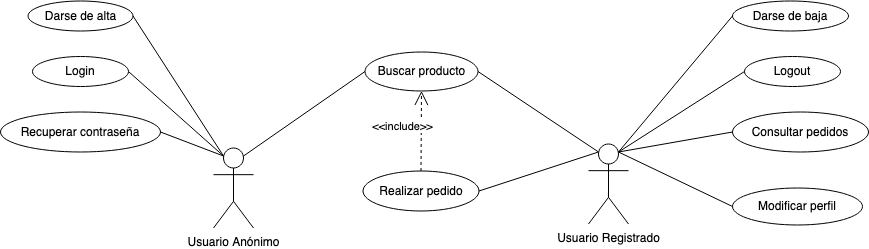
\includegraphics[width=\textwidth]{use-case_diagram}
                \caption{Diagrama de casos de uso}
                \label{fig:use-case_diagram}
            \end{figure}

            \paragraph{CU01\_Búsqueda}
            Proceso por el cual un usuario explora el catálogo y acaba por visualizar la página de un libro.
            \begin{itemize}
                \item[+] Actores implicados: Usuario Anónimo, Usuario Registrado.
                \item[+] Precondiciones: Usuario situado en cualquiera de las páginas que dan acceso al catálogo.
                \item[+] Flujo principal:
                \begin{enumerate}
                    \item[1.] El usuario hace click en alguna de las categorías principales mostradas a modo de catálogo flotante en la barra de navegación
                    o hace click en \emph{All Books}.
                    \item[2.] El sistema muestra la página de resultados de búsqueda.
                    \item[3.] El usuario hace click en alguno de los productos mostrados.
                    \item[4.] El sistema muestra la página del libro.
                \end{enumerate}
                \item[+] Flujo alternativo: \emph{refinamiento\_búsqueda}. El usuario altera en la página de resultados algún criterio de filtro.
                \begin{itemize}
                    \item[3.b.] El usuario selecciona/deselecciona algún criterio de filtro de entre los mostrados en la página de resultados de búsqueda.
                    \item[4.b.] El sistema vuelve al punto 2 del flujo principal.
                \end{itemize}
                \item[+] Flujo alternativo: \emph{búsqueda\_por\_texto}. El usuario introduce una cadena de texto en el cuadro de búsqueda.
                \begin{itemize}
                    \item[1.b.] El usuario introduce una cadena de texto en el cuadro de búsqueda y hace click en buscar.
                \end{itemize}
            \end{itemize}

            \paragraph{CU02\_Alta}
            Proceso por el cual se crea un nuevo usuario registrado.
            \begin{itemize}
                \item[+] Actores implicados: Usuario Anónimo.
                \item[+] Flujo principal:
                \begin{enumerate}
                    \item[1.] El usuario hace click en el link de nuevo registro, disponible en la página de \emph{login}.
                    \item[2.] El sistema presenta un formulario donde introducir la dirección de email y la contraseña.
                    \item[3.] El usuario introduce y envía la información pedida.
                    \item[4.] El sistema comprueba la información proporcionada.
                    \item[5.] El sistema crea una nueva cuenta de usuario, pero la mantiene inactiva a la espera de confirmar la dirección de email.
                    \item[6.] El sistema envía un email con un link de confirmación a la dirección proporcionada, e informa al usuario por pantalla.
                    \item[7.] El usuario accede a su email y hace click en el link enviado, confirmando que la dirección de email es suya.
                    \item[8.] El sistema activa la cuenta de usuario.
                    \item[9.] El sistema envía al usuario un email de bienvenida.
                    \item[10.] El sistema redirige al usuario a la página de \emph{login}.
                \end{enumerate}
                \item[+] Flujo alternativo: \emph{usuario\_ya\_registrado}. La dirección proporcionada se encuentra registrada en el sistema.
                \begin{itemize}
                    \item[5.b.] El sistema no crea una nueva cuenta de usuario. Por razones de seguridad, la manera en que el sistema informa al usuario tras esta situación es indistinguible del flujo principal, de forma que no se pueda deducir que ese email ya tiene cuenta asociada en el sistema.
                \end{itemize}
                \item[+] Flujo alternativo: \emph{link\_ya\_enviado}. El sistema está a la espera de la confirmación de un link válido en esta dirección de email.
                \begin{itemize}
                    \item[5.b.] El sistema no crea una nueva cuenta de usuario. Se informa al usuario acerca de una condición de error \-{}genérica, por seguridad\- en relación con la dirección de email proporcionada, pidiéndose que compruebe su dirección de email.
                \end{itemize}
                \item[+] Flujo excepcional: \emph{time\_out}. El usuario no confirma su dirección de email dentro de un plazo determinado.
                \begin{itemize}
                    \item[7.b.] El sistema detecta el timeout e invalida el link de confirmación enviado. Si el usuario hace click en el link caducado se le informa de dicha condición.
                \end{itemize}
            \end{itemize}

            \paragraph{CU03\_Login}
                Proceso por el cual un usuario se autentica en el sistema.
                \begin{itemize}
                    \item[+] Actores implicados: Usuario Anónimo.
                    \item[+] Flujo principal:
                    \begin{enumerate}
                        \item[1.] El usuario hace click en el link de \emph{login}, o intenta realizar alguna operación que requiera autenticación (por ejemplo, añadir un libro a la cesta).
                        \item[2.] El sistema presenta el formulario de acceso (dirección de email y la contraseña).
                        \item[3.] El usuario introduce y envía la información pedida.
                        \item[4.] El sistema comprueba las credenciales.
                        \item[5.] El sistema redirige al usuario a la página principal.
                    \end{enumerate}
                    \item[+] Flujo alternativo: \emph{fallo\_autenticación}. El email no se encuentra registrado en el sistema, o la contraseña proporcionada no es correcta.
                    \begin{itemize}
                        \item[5.b.] El sistema informa al usuario acerca de un fallo genérico de autenticación, de forma que, por razones de seguridad, no se pueda deducir si el email proporcionado se encuentra registrado en el sistema.
                    \end{itemize}
                    \item[+] Flujo alternativo: \emph{bloqueo\_cuenta}. El usuario anónimo realiza, dentro de un marco de tiempo (configurable), un número de intentos (configurable) de login con contraseña errónea.
                    \begin{itemize}
                        \item[5.b.] El sistema bloquea la cuenta asociada al email para prevenir ataques por fuerza bruta.
                        \item[6.] El sistema informa al usuario por pantalla y mediante el envío de un email.
                        \item[7.] Pasado el tiempo de seguridad (configurable), el sistema desbloquea la cuenta del usuario.
                    \end{itemize}
                    \item[+] Post-Condiciones: El usuario pasa a tener rol de usuario registrado en el sistema.
                \end{itemize}

            \paragraph{CU04\_RecuperarContraseña}
                Un usuario previamente registrado en el sistema intenta acceder al mismo, pero no recuerda su contraseña. El sistema intentará crear una nueva contraseña y enviarla al e-mail del usuario.
                \begin{itemize}
                    \item[+] Actores implicados: Usuario Anónimo.
                    \item[+] Flujo principal:
                    \begin{enumerate}
                        \item El usuario hace click en la opción \emph{¿olvidó su contraseña?}.
                        \item El sistema presenta un formulario donde introducir la dirección de email.
                        \item El usuario introduce y envía su dirección de email.
                        \item El sistema comprueba la dirección de email.
                        \item Comprobación correcta. El sistema envía un email con un link de confirmación a la dirección proporcionada, e informa de ello al usuario por pantalla.
                        \item Link no caducado. El usuario accede a su email y hace click en el link, confirmando que efectivamente la dirección proporcionada es la suya.
                        \item El sistema genera una nueva contraseña y se la asigna al usuario.
                        \item El sistema envía la nueva contraseña a la dirección de email del usuario, y le avisa de ello por pantalla.
                    \end{enumerate}
                    \item[+] Flujo alternativo: \emph{usuario\_no\_registrado}. La dirección proporcionada no se encuentra registrada en el sistema.
                    \begin{itemize}
                        \item[5.b.] El sistema no envía correo alguno pero, por razones de seguridad, desde el punto de vista del usuario este flujo alternativo es indistinguible del principal.
                    \end{itemize}
                    \item[+] Flujo excepcional: \emph{time\_out}. El usuario no confirma su dirección de email dentro de un plazo determinado.
                    \begin{itemize}
                        \item[6.b.] El sistema detecta el timeout e invalida el link de confirmación enviado. Si el usuario hace click en el link caducado se le informara de dicha condición.
                    \end{itemize}
                \end{itemize}

            \paragraph{CU05\_EditarPerfil}
                Proceso por el cual un usuario modifica alguno de los datos de su perfil personal.
                \begin{itemize}
                    \item[+] Actores implicados: Usuario Registrado.
                    \item[+] Flujo principal:
                    \begin{enumerate}
                        \item[1.] El usuario hace click en \emph{área personal}.
                        \item[2.] El sistema muestra la página de área personal, en donde se muestra el formulario de datos personales, rellenado con la información actual del usuario.
                        \item[3.] El usuario modifica los datos del formulario y lo envía al sistema.
                        \item[4.] El sistema comprueba los datos.
                        \item[5.] Comprobación correcta.El sistema actualiza la información del usuario.
                        \item[6.] El sistema muestra la página de inicio.
                    \end{enumerate}
                    \item[+] Flujo alternativo: \emph{error\_datos\_formulario}. Los datos proporcionados en el formulario de información personal no son válidos.
                    \begin{itemize}
                        \item[5.b.] El sistema regresa al punto 3 del flujo principal, e informa al usuario acerca del fallo producido.
                    \end{itemize}
                    \item[+] Flujo alternativo: \emph{cancelar}. El usuario cancela el proceso de edición de su información personal.
                    \begin{itemize}
                        \item[3.b.] El usuario hace click en el botón \emph{cancelar}. El sistema muestra la página de inicio.
                    \end{itemize}
                    \item[+] Post-Condiciones: El usuario ha alterado su información personal almacenada en la aplicación.
                \end{itemize}

            \paragraph{CU06\_RealizarPedido}
                Proceso por el cual un usuario realiza una compra a través de la aplicación web.
                \begin{itemize}
                    \item[+] Actores implicados: Usuario Registrado.
                    \item[+] Precondiciones: Desde cualquier página en la que se muestren libros (página de inicio, página de resultados de búsqueda o página de un libro) el usuario hace click en \emph{add to cart}, para uno o mas libros.
                    \item[+] Flujo principal:
                    \begin{enumerate}
                        \item[1.] El usuario hace click en el icono de la cesta.
                        \item[2.] El sistema muestra la página de la cesta del usuario, con todos los libros contenidos en el mismo.
                        \item[3.] El usuario puede aumentar o disminuir el número de unidades de un libro, o incluso eliminarlo por completo, y hace click en \emph{checkout}.
                        \item[4.] El sistema comprueba la disponibilidad de los libros contenidos en la cesta.
                        \item[5.] Stock suficiente. El sistema muestra la página de checkout, con el formulario de datos de envío y pago, y el resumen de la compra.
                        \item[6.] El usuario completa los datos de envío y de pago y hace click en \emph{Pay}.
                        \item[7.] El sistema tramita el pago.
                        \item[8.] Pago ok. El sistema registra el nuevo pedido.
                        \item[9.] El sistema confirma al usuario por pantalla y por email que el pedido se ha realizado con éxito.
                    \end{enumerate}
                    \item[+] Flujo alternativo: \emph{stock\_insuficiente}. No hay stock suficiente para satisfacer el contenido de la cesta.
                    \begin{itemize}
                        \item[5.b.] El sistema vuelve al punto 2 del flujo principal, informando al usuario de los libros para los cuales no hay stock suficiente.
                        \item[3.b.] El usuario reduce la cantidad demandada de los libros correspondientes y hace click en \emph{checkout}.
                    \end{itemize}
                    \item[+] Flujo alternativo: \emph{error\_pago}. Error al efectuar el pago.
                    \begin{itemize}
                        \item[8.b.] El sistema vuelve al punto 5 del flujo principal, informando al usuario del problema respecto al pago.
                    \end{itemize}
                    \item[+] Flujo excepcional: \emph{libro\_eliminado}. Algún libro de la cesta ya no esta disponible en el sistema.
                    \begin{itemize}
                        \item[5.b.] El sistema elimina de la cesta automáticamente los libros que el administrador haya deshabilitado.
                        \item[6.b.] El sistema vuelve al punto 2 del flujo principal, informando al usuario de los libros que han sido eliminados.
                    \end{itemize}
                    \item[+] Post-Condiciones: El usuario ha efectuado un nuevo pedido.
                \end{itemize}

            \paragraph{CU07\_ConsultarPedido}
                Proceso por el cual un usuario consulta el historial de pedidos que ha realizado.
                \begin{itemize}
                    \item[+] Actores implicados: Usuario Registrado.
                    \item[+] Flujo principal:
                    \begin{enumerate}
                        \item[1.] El usuario hace click en \emph{My Purchases} en la barra de navegación.
                        \item[2.] El sistema muestra la página de los pedidos del usuario.
                        \item[3.] El usuario puede expandir-contraer la información mostrada relativa a un pedido.
                    \end{enumerate}
                \end{itemize}

            \paragraph{CU08\_Baja}
                Proceso por el cual un usuario elimina su cuenta de la tienda online.
                \begin{itemize}
                    \item[+] Actores implicados: Usuario Registrado.
                    \item[+] Flujo principal:
                    \begin{enumerate}
                        \item[1.] El usuario hace click en \emph{área personal}.
                        \item[2.] El sistema muestra la página de área personal.
                        \item[3.] El usuario selecciona \emph{eliminar cuenta}.
                        \item[4.] El sistema muestra el formulario de eliminación de cuenta.
                        \item[5.] El usuario completa y envía el formulario.
                        \item[6.] El sistema comprueba los datos.
                        \item[7.] Comprobación correcta. El sistema actualiza el estado del usuario y envía un email de confirmación.
                        \item[8.] El sistema muestra la página de inicio.
                    \end{enumerate}
                    \item[+] Flujo alternativo: \emph{error\_datos\_formulario}. La contraseña proporcionada en el formulario de baja no es correcta.
                    \begin{itemize}
                        \item[7.b.] El sistema regresa al punto 4 del flujo principal, e informa al usuario acerca del fallo producido.
                    \end{itemize}
                    \item[+] Flujo alternativo: \emph{cancelar}. El usuario cancela el proceso de baja.
                    \begin{itemize}
                        \item[5.b.] El usuario cancela el proceso de baja. El sistema regresa al punto 2 del flujo principal.
                    \end{itemize}
                    \item[+] Post-Condiciones: El usuario ya no figura como dado de alta en la aplicación.
                \end{itemize}

            \paragraph{CU09\_Logout}
                Proceso por el cual un usuario cierra su sesión en el sistema.
                \begin{itemize}
                    \item[+] Actores implicados: Usuario Registrado.
                    \item[+] Precondiciones: el usuario está con su sesión abierta en el sistema.
                    \item[+] Flujo principal:
                    \begin{enumerate}
                        \item[1.] El usuario hace click en el link de \emph{logout}.
                        \item[2.] El sistema cierra la sesión del usuario.
                        \item[3.] El sistema muestra la página de inicio.
                    \end{enumerate}
                    \item[+] Post-Condiciones: El usuario ha efectuado el logout con éxito.
                \end{itemize}